\documentclass{report}
\usepackage{makeidx}
\usepackage{graphicx}
\usepackage{subfigure}
\usepackage{titlesec}
\usepackage{fullpage}
\setcounter{secnumdepth}{4}
\usepackage[utf8]{inputenc}
\usepackage{import}
\usepackage{doxygen}
\usepackage{hyperref}
\usepackage{amsmath,diagbox,ifthen}

\title{mycc - My own C++ compiler implementation}
\author{Hanze Chen}
\date{January 2022}
\makeindex

%% doxygen fix
\newcommand{\+}{}


\begin{document}
    \maketitle


    \section{Introduction}\label{sec:introduction}
    \begin{figure}[hb!]
        \centering
        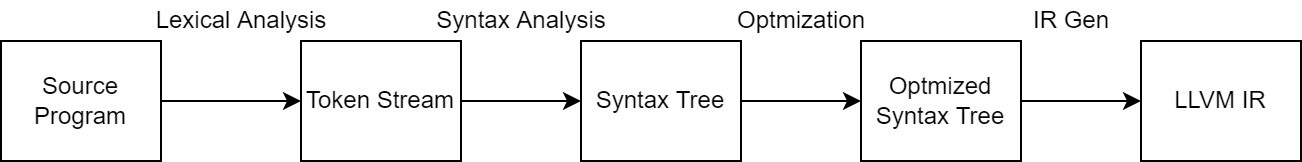
\includegraphics[width=10cm]{figure/frontend_structure}
        \caption{Frontend Structure}
        \label{fig:frontend_structure}
    \end{figure}


    \section{Implemented Function}\label{sec:implemented-function}

    \subsection{Part0}\label{subsec:part0}
    When part 0 is enabled by "-0" option.
    The compiler will only generate the output like Figure~\ref{fig:example_part0_output} Shows: \par
    \begin{figure}[hb!]
        \centering
        \fbox{
            \shortstack[l]{
                My bare-bones C compiler (for COM 440/540) \\
                Written by Hanze Chen (hanzech@iastate.edu) \\
                Version 0.1.0\_9c370c3(WorkStation) \\
                2022-01-28 13:18:14
            }
        }
        \caption{Example Output for Part 0}
        \label{fig:example_part0_output}
    \end{figure}

    Version string is in format of Major\_Minor\_Patch\_Commit Hash(compile machine's hostname). And the last line is
    the build time. In my implantation those variables will generate when CMake projects is finished its configuration
    step. And those variable will be run-time accessible via “version.h" which will generate by CMake from "version.h.in" \par

    When compiler is running in part 0 mode (with "-0" flag), the compiler will not process any input file, and will
    always write the version message like Figure~\ref{fig:example_part0_output} to output file (declared by "-o" flag)

    \subsection{Part1}\label{subsec:part1}
    Part1 will be enabled by adding "-1" option. The compiler will print the lexer parsing result to stdout if no output
    files is assigned. Any error generated by lexer will directly print to stderr. The example correct output is like
    Figure\ref{fig:example_part1_output}, the compiler takes hello.c[Figure] as input, then its output will contains all
    token which lexer parsed[Figure\ref{fig:example_part1_output}]. The lexer's output will strictly followed the
    following format:
    \begin{quote}
    {\texttt{where} File}
        \emph{filename}
        {\texttt{\emph{line number}
        {\texttt{\emph{token number}
        {\texttt{\emph{lexeme}} Text}} Token}} Line}
    \end{quote}

    \begin{itemize}
        \item \emph{filename}
        is the name of the input file that contains the token,
        \item \emph{line number}
        is the line number of the input file that contains the token,
        \item \emph{token number}
        is the integer corresponding to the token, given in \verb|tokens.h|
        and Table~\ref{tab:tokens}, and
        \item \emph{lexeme}
        is the matched text that produced the token.
    \end{itemize}

    In my implantation, there will be two different error output styles, the basic output format is exactly have the form like:
    \begin{quote}
        \begin{tabbing}
        {\texttt{} Lexer}
            \= {\texttt{\emph{filename}
            {\texttt{\emph{line number}
            {\texttt{\emph{lexeme}} near text}} line}} error in file}
            \\
            \> \emph{Description}
        \end{tabbing}
    \end{quote}

    \begin{figure}[hb!]
        \centering
        \fbox{
            \shortstack[l]{
                File hello.c Line 8 Token 301 Text int\\
                File hello.c Line 8 Token 306 Text main\\
                File hello.c Line 8 Token 40 Text (\\
                File hello.c Line 8 Token 41 Text )\\
                File hello.c Line 9 Token 123 Text \{\\
                File hello.c Line 10 Token 410 Text return\\
                File hello.c Line 10 Token 306 Text printf\\
                File hello.c Line 10 Token 40 Text (\\
                File hello.c Line 10 Token 305 Text "Hello, world!"\\
                File hello.c Line 10 Token 41 Text )\\
                File hello.c Line 10 Token 59 Text ;\\
                File hello.c Line 11 Token 125 Text \}
            }
        }
        \caption{Part1 example output}
        \label{fig:example_part1_output}
    \end{figure}


    \subsection{Part3}\label{subsec:part3}
    Part3 will be enabled by adding "-3" option. The compiler will print the syntax parsing result to stdout if no output
    files is assigned. Any error generated by lexer will directly print to stderr. The example correct output is like
    Figure\ref{fig:example_part2_output}, the compiler takes hello.c[Figure] as input, then its output will contains all
    token which lexer parsed[Figure\ref{fig:example_part2_output}]. The lexer's output will strictly followed the
    following format:
    When executed with a mode of thispart, your compiler should read the specified input file and check that the file has correct C syntax . If the input file is not syntactically correct, then display an appropriate error message. Error messages should be written to standard error, and have the format
    \begin{quote}
        \begin{tabbing}
        {\tt Parser }
            \={\tt error in file }\emph{filename}
            {\tt line }\emph{line number}
            {\tt near text }\emph{lexeme}
            \\
            \> \emph{Description}
        \end{tabbing}
    \end{quote}
    where the line number and offending text should be where the error occurs (or was detected). The description will typically indicate what the parser expected to appear next in input. After the first syntax error, your parser may either make a ``best effort'' attempt to continue processing the input file, or exit. When tested on input files with syntax errors, your compiler will be considered correct if it catches the first syntax error. If the input file is syntactically correct, then simply write
    \begin{quote}
        \verb|File| \emph{filename} \verb|is syntactically correct.|
    \end{quote}
    to the output stream.

    We are using following precedence and associative of operations:
    \begin{table}[t]
        \begin{center}
            \begin{tabular}{@{}l|c|c}
                \hline
                \multicolumn{1}{c|}{\sc Operators}
                &
                    {\sc Associativity}
                &
                    {\sc Precedence}
                \\ \hline
                \verb|()| \quad \verb|[]| \quad .
                &
                left to right
                &
                (highest)
                \\
                \verb|!| \quad \verb|~| \quad \verb|-| (unary)
                \quad \verb|--| \quad \verb|++|
                % \quad \verb|&| (unary)
                \quad \verb|(|\emph{type}\verb|)|
                &
                right to left
                \\
                \verb|*| \quad \verb|/| \quad \verb|%|
                &
                left to right
                \\
                \verb|+| \quad \verb|-|
                &
                left to right
                \\
                \verb|<| \quad \verb|<=| \quad \verb|>| \quad \verb|>=|
                &
                left to right
                \\
                \verb|==| \quad \verb|!=|
                &
                left to right
                \\
                \verb|  &  |
                &
                left to right
                \\
                \verb$|$
                &
                left to right
                \\
                \verb|  &   &  |
                &
                left to right
                \\
                \verb$||$
                &
                left to right
                \\
                \verb$?:$
                &
                right to left
                \\
                \verb|=| \quad \verb|+=| \quad \verb|-=| \quad \verb|*=| \quad \verb|/=|
                &
                right to left
                \\
                \verb|,|
                &
                left to right
                &
                (lowest)
                \\ \hline
            \end{tabular}
        \end{center}
        \caption{Precedence and associativity of operators}
        \label{TAB:precedence}
    \end{table}


    \section{Component}\label{sec:component}

    \subsection{Lexical}\label{subsec:lexical}
    \begin{table}[t]
        \centering
        \begin{tabular}{rlcrlcrl}
            \multicolumn{8}{c}{Single character symbols}
            \\[1mm]
            {\bf Value} & {\bf Lexeme}
            & ~~~~~~ &
                {\bf Value} & {\bf Lexeme}
            & ~~~~~~ &
                {\bf Value} & {\bf Lexeme}
            \\ \cline{1-2} \cline{4-5} \cline{7-8}
            33 & \verb|!| & &
            37 & \verb|%| & &
            38 & \verb|  &  | \\
            40 & \verb|(| & &
            41 & \verb|)| & &
            42 & \verb|*| \\
            43 & \verb|+| & &
            44 & \verb|,| & &
            45 & \verb|-| \\
            46 & \verb|.| & &
            47 & \verb|/| & &
            58 & \verb|:| \\
            59 & \verb|;| & &
            60 & \verb|<| & &
            61 & \verb|=| \\
            62 & \verb|>| & &
            63 & \verb|?| & &
            91 & \verb|[| \\
            93 & \verb|]| & &
            123 & \verb|{| & &
            124 & \verb+|+ \\
            125 & \verb|}| & &
            126 & \verb|~| \\
            \\
            \multicolumn{8}{c}{Operators with two characters}
            \\[1mm]
            {\bf Value} & {\bf Lexeme}
            & ~~~~~~ &
                {\bf Value} & {\bf Lexeme}
            & ~~~~~~ &
                {\bf Value} & {\bf Lexeme}
            \\ \cline{1-2} \cline{4-5} \cline{7-8}
            351 & \verb|==| & &
            352 & \verb|!=| & &
            353 & \verb|>=| \\
            354 & \verb|<=| & &
            355 & \verb|++| & &
            356 & \verb|--| \\
            357 & \verb+||+ & &
            358 & \verb|&  &  | & &
            361 & \verb|+=| \\
            362 & \verb|-=| & &
            363 & \verb|*=| & &
            364 & \verb|/=| \\
            \\
            \multicolumn{8}{c}{Keywords}
            \\[1mm]
            {\bf Value} & {\bf Lexeme}
            & ~~~~~~ &
                {\bf Value} & {\bf Lexeme}
            & ~~~~~~ &
                {\bf Value} & {\bf Lexeme}
            \\ \cline{1-2} \cline{4-5} \cline{7-8}
            401 & \verb|const| & &
            402 & \verb|struct| & &
            403 & \verb|for| \\
            404 & \verb|while| & &
            405 & \verb|do| & &
            406 & \verb|if| \\
            407 & \verb|else| & &
            408 & \verb|break| & &
            409 & \verb|continue| \\
            410 & \verb|return| & &
            411 & \verb|switch| & &
            412 & \verb|case| \\
            413 & \verb|default| \\
        \end{tabular}

        \begin{tabular}{rll}
            \\
            \multicolumn{3}{c}{Lexemes with attributes}
            \\[1mm]
            {\bf Value} & {\bf Lexeme} & {\bf Definition}
            \\ \hline
            301 & type & \verb|void| or \verb|char| or \verb|int| or \verb|float|
            \\
            302 & character literal & a character enclosed in single quotes;
            escape sequences are extra credit
            \\
            303 & integer literal & a sequence of one or more digits
            \\
            304 & real literal & two sequences each of one or more digits, separated by \verb|.|
            \\
            305 & string literal & a sequence of zero or more characters (including escape sequences,
            \\ & & except for \verb|\\| and \verb|\"|) enclosed in double quotes
            \\
            306 & identifier & a letter or underscore, followed by zero or more letters,
            underscores, or
            \\ & & digits, that is not a keyword or type
        \end{tabular}

        \caption{Tokens to be recognized by the lexer.}
        \label{tab:tokens}
    \end{table}


    \section{Main Data Structures}\label{sec:main-data-structures}

    \subsection{Lexical}\label{subsec:lexical2}

    \subsubsection{StringToken \index{String Token Class}}
    Recall the compiler frontend workflow described in Figure~\ref{fig:frontend_structure}. TokenStream is defined as
    a list of StringToken class which contains all parsed available token in source file.\par
    Currently all the supported lexical token type and its regex expression is included in Table~\ref{tab:supported_lexical_token_list}: \par
    \begin{table}[hb!]
        \centering
        \begin{tabular}{l|lll}
            \hline
            Token Type   & Regex                                                  & Example           & Description    \\ \hline
            Add          & \textbackslash{}\textbackslash{}+                      & +                 & Addition       \\
            Sub          & -                                                      & -                 & Subtraction    \\
            Mul          & \textbackslash{}\textbackslash{}*                      & *                 & Multiplication \\
            Div          & /                                                      & /                 & Division       \\
            Mod          & \%                                                     & \%                & Modulus        \\
            Assign       & =                                                      & =                 & Assignment     \\
            Exclamatory  & !                                                      & !                 & Exclamation    \\
            LBracket     & \textbackslash{}\textbackslash{}(                      & (                 & Left Bracket   \\
            RBracket     & \textbackslash{}\textbackslash{}(                      & )                 & Right Bracket  \\
            LBrace       & \textbackslash{}\{                                     & \{                & Left Brace     \\
            RBrace       & \textbackslash{}\}                                     & \}                & Right Brace    \\
            Comma        & ,                                                      & ,                 & Comma          \\
            Semicolon    & ;                                                      & ;                 & Semicolon      \\
            Colon        & :                                                      & :                 & Colon          \\
            Dot          & \textbackslash{}\textbackslash{}.                      & .                 & Dot            \\
            Greater      & \textgreater{}                                         & \textgreater{}    & Greater        \\
            Less         & \textless{}                                            & \textless{}       & Less           \\
            LBound       & \textbackslash{}[                                      & {]}               & Left Bound     \\
            RBound       & \textbackslash{}]                                      & {[}               & Right Bound    \\
            QuestionMark & \textbackslash{}\textbackslash{}?                      & ?                 & Question Mark  \\
            Esperluette  & \textbackslash{}\&                                     & \&                & Esperluette    \\
            Star         & \textbackslash{}\textbackslash{}*                      & *                 & Star           \\
            VerticalBar  & \textbackslash{}\textbackslash{}|                      & |                 & Vertical Bar   \\
            number       & {[}0-9{]}+\textbackslash{}\textbackslash{}.?{[}0-9{]}* & 0, 0.1 etc.       & Numbers        \\
            Identifiers  & {[}a-zA-Z\_{]}{[}a-zA-Z0-9\_{]}*                       & "a", "while" etc. & Identifiers    \\ \hline
        \end{tabular}
        \caption{Supported String Token Type}
        \label{tab:supported_lexical_token_list}
    \end{table}

    \subsection{Utils}\label{subsec:utils}

    \subsubsection{Status \index{Status Class}}


    \section{User Manual}\label{sec:user-manual}

    \appendix


    \section{API reference }
    \subimport{latex/}{refman.tex}

    \printindex
\end{document}


